\documentclass{memoir}
\usepackage{amsmath}
\usepackage[utf8]{inputenc}
\usepackage[english]{babel}
\usepackage{csquotes}
\usepackage{makeidx}
\usepackage{showidx}
\usepackage{listings}
\usepackage{tikz}
\makeindex
\usepackage[backend=biber]{biblatex}
\addbibresource{../../doc/doc.bib}

\usetikzlibrary{positioning,calc,fit}
\definecolor{mybluei}{RGB}{124,156,205}
\definecolor{myblueii}{RGB}{73,121,193}
\definecolor{mygreen}{RGB}{202,217,126}
\definecolor{mypink}{RGB}{233,198,235}

% this length is used to control the width of the light blue frame
% for the upper part of the diagram
\newlength\myframesep
\setlength\myframesep{8pt}

\pgfdeclarelayer{background}
\pgfsetlayers{background,main}

\pgfkeys{
	/tikz/node distance/.append code={
		\pgfkeyssetvalue{/tikz/node distance value}{#1}
	}
}

\newcommand\widernode[5][blueb]{
	\node[
	#1,
	inner sep=0pt,
	shift=($(#2.south)-(#2.north)$),
	yshift=-\pgfkeysvalueof{/tikz/node distance value},
	fit={(#2) (#3)},
	label=center:{\sffamily\bfseries\color{white}#4}] (#5) {};
}


\title{Ugarit Manual}
\author{Christian Kotz}
\date{\today}

\begin{document}

\index{Cpp}

\autocite{ISO/IEC2020}

\section{Architecture}

Ugarit use a layered architecture. Each layer forms a  partition within module \lstinline!ugarit!.

\begin{figure}
	\centering
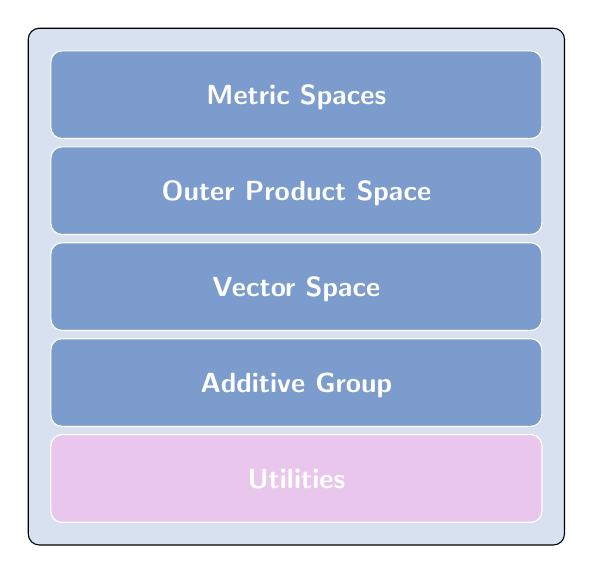
\begin{tikzpicture}[node distance=3pt,outer sep=0pt,
	blueb/.style={
		draw=white,
		fill=mybluei,
		rounded corners,
		text width=6cm,
		font={\sffamily\bfseries\color{white}},
		align=center,
		text height=16pt,
		text depth=9pt},
	greenb/.style={blueb,fill=mygreen},
	]
	\node[blueb] (MS) { Metric Spaces };
	\node[blueb, below=of MS] (OS) {Outer Product Space};
	\node[blueb, below=of OS] (VS) {Vector Space};
	\node[blueb, below=of VS] (AG) {Additive Group};
	\node[blueb, below=of AG] (CTS) {Compile-time Sparse Vectors};	
	\begin{pgfonlayer}{background}
		\draw[blueb,draw=black,fill=mybluei!30] 
		([xshift=-8pt,yshift=8pt]current bounding box.north west) rectangle 
		([xshift=8pt,yshift=-8pt]current bounding box.south east);
	\end{pgfonlayer}	
	
	\node[blueb,fill=mypink, below=of AG] (UTIL) {Utilities};	
\end{tikzpicture}
\caption{layered architecture}
\end{figure};
 
\printbibliography

\end{document}
